\documentclass[tikz]{standalone}
\usepackage{tikz}
\usepackage{pgfplots} % for tikz plot
\usetikzlibrary{positioning,fit,calc,shadows}

% \pgfrealjobname{dummy}

\begin{document}

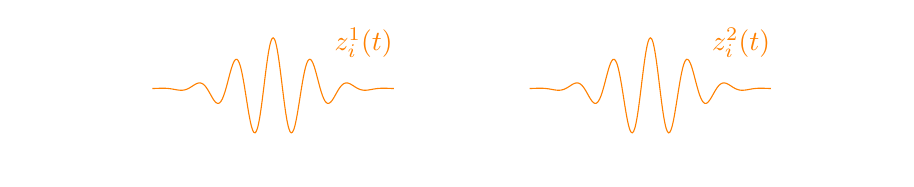
\begin{tikzpicture}[/pgfplots/.cd,width=\columnwidth,height=3cm]
    \begin{axis}[xmin=-0.5,xmax=5,ymin=-1,ymax=1.2,
        xticklabels=\empty,
        yticklabels=\empty,
        axis line style={draw=none},
        tick style={draw=none}]
        %\addplot[no markers,smooth,samples=201,domain=0:2.5, color=white] 
        {exp(-9*(x-1)*(x-1))*cos((x-1)*1440)};

        %\addplot[no markers,smooth,samples=401,domain=0:5, color=white] 
        %{exp(-9*(x-1)*(x-1))*cos((x-1)*1440) + exp(-9*(x-3.5)*(x-3.5))*cos((x-3.5)*1440)};
        %\addplot[no markers,smooth,samples=201,domain=0.2:1.8, color=orange] 
        {exp(-9*(x-1)*(x-1))*cos((x-1)*1440)};
        %\addplot[no markers,smooth,samples=201,domain=2.7:4.3, color=orange] 
        {exp(-9*(x-3.5)*(x-3.5))*cos((x-3.5)*1440)};
        % 

        \addplot[no markers,smooth,samples=2,domain=0:0.2, color=white]
        {exp(-9*(x-1)*(x-1))*cos((x-1)*1440) + exp(-9*(x-3.5)*(x-3.5))*cos((x-3.5)*1440)}; 
        \addplot[no markers,smooth,samples=201,domain=0.2:1.8, color=orange]
        {exp(-9*(x-1)*(x-1))*cos((x-1)*1440) + exp(-9*(x-3.5)*(x-3.5))*cos((x-3.5)*1440)};
        \addplot[no markers,smooth,samples=2,domain=1.8:2.7, color=white]
        {exp(-9*(x-1)*(x-1))*cos((x-1)*1440) + exp(-9*(x-3.5)*(x-3.5))*cos((x-3.5)*1440)};
        \addplot[no markers,smooth,samples=201,domain=2.7:4.3, color=orange]
        {exp(-9*(x-1)*(x-1))*cos((x-1)*1440) + exp(-9*(x-3.5)*(x-3.5))*cos((x-3.5)*1440)};
        \addplot[no markers,smooth,samples=2,domain=4.3:5, color=white]
        {exp(-9*(x-1)*(x-1))*cos((x-1)*1440) + exp(-9*(x-3.5)*(x-3.5))*cos((x-3.5)*1440)};

        {exp(-9*(x-1)*(x-1))*cos((x-1)*1440) + exp(-9*(x-3.5)*(x-3.5))*cos((x-3.5)*1440)};


        \node[text=orange] at (axis cs:1.6,0.9) {$z_i^1(t)$};
        \node[text=orange] at (axis cs:4.1,0.9) {$z_i^2(t)$};
        \node[color=white] at (axis cs:-0.1,0.4) {$y_i(t)$};

        %\node[color=white] at (axis cs:0.2,-0.3) {$ $};
        %\node[] at (axis cs:0.2,0) {$|$};
        %\node[] at (axis cs:1.8,0) {$|$};
        %\node[color=white] at (axis cs:2.7,-0.3) {$ $};
        %\node[] at (axis cs:2.7,0) {$|$};
        %\node[] at (axis cs:4.3,0) {$|$};

    \end{axis}
\end{tikzpicture}

\begin{tikzpicture}[/pgfplots/.cd,width=\columnwidth,height=3cm]
    \begin{axis}[xmin=-0.5,xmax=5,ymin=-1,ymax=1.2,
        xticklabels=\empty,
        yticklabels=\empty,
        axis line style={draw=none},
        tick style={draw=none}]
        \addplot[no markers,smooth,samples=201,domain=0:2.5, color=white] 
        {exp(-9*(x-1)*(x-1))*cos((x-1)*1440)};

        \addplot[no markers,smooth,samples=201,domain=2.5:5, color=white] 
        {exp(-9*(x-3.5)*(x-3.5))*cos((x-3.5)*1440)};
        \addplot[no markers,smooth,samples=201,domain=0.2:1.8, color=orange] 
        {exp(-9*(x-1)*(x-1))*cos((x-1)*1440)};
        %\addplot[no markers,smooth,samples=201,domain=2.7:4.3, color=orange] 
        {exp(-9*(x-3.5)*(x-3.5))*cos((x-3.5)*1440)};
        % 
        \node[text=orange] at (axis cs:1.6,0.9) {$z_i^1(t)$};
        %\node[text=orange] at (axis cs:4.1,0.9) {$z_i^2(t)$};
        \node[color=white] at (axis cs:-0.1,0.4) {$y_i(t)$};

        \node[color=white] at (axis cs:0.2,-0.3) {$ $};
        \node[color=white] at (axis cs:0.2,0) {$|$};
        \node[color=white] at (axis cs:2.7,-0.3) {$ $};
        %\node[] at (axis cs:2.7,0) {$|$};
    \end{axis}
\end{tikzpicture}

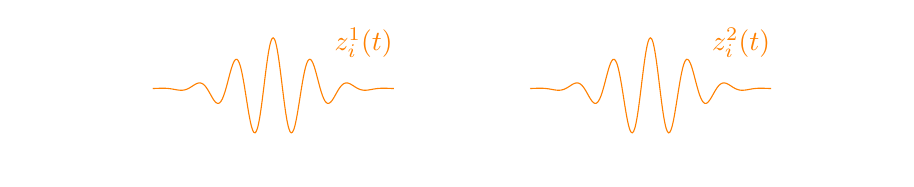
\begin{tikzpicture}[/pgfplots/.cd,width=\columnwidth,height=3cm]
    \begin{axis}[xmin=-0.5,xmax=5,ymin=-1,ymax=1.2,
        xticklabels=\empty,
        yticklabels=\empty,
        axis line style={draw=none},
        tick style={draw=none}]
        \addplot[no markers,smooth,samples=201,domain=0:2.5, color=white] 
        {exp(-9*(x-1)*(x-1))*cos((x-1)*1440)};

        \addplot[no markers,smooth,samples=201,domain=2.5:5, color=white] 
        {exp(-9*(x-3.5)*(x-3.5))*cos((x-3.5)*1440)};
        \addplot[no markers,smooth,samples=201,domain=0.2:1.8, color=orange] 
        {exp(-9*(x-1)*(x-1))*cos((x-1)*1440)};
        \addplot[no markers,smooth,samples=201,domain=2.7:4.3, color=orange] 
        {exp(-9*(x-3.5)*(x-3.5))*cos((x-3.5)*1440)};
        % 
        \node[text=orange] at (axis cs:1.6,0.9) {$z_i^1(t)$};
        \node[text=orange] at (axis cs:4.1,0.9) {$z_i^2(t)$};
        \node[color=white] at (axis cs:-0.1,0.4) {$y_i(t)$};

        \node[color=white] at (axis cs:0.2,-0.3) {$ $};
        \node[color=white] at (axis cs:0.2,0) {$|$};
        \node[color=white] at (axis cs:2.7,-0.3) {$ $};
        \node[color=white] at (axis cs:2.7,0) {$|$};
    \end{axis}
\end{tikzpicture}

\begin{tikzpicture}[typetag/.style={rectangle, draw, rounded corners,fill=black!70, fill opacity=1, text opacity=1,text width=1.4cm, align=center,minimum width=1cm, minimum height=0.5cm},
    cascaded/.style={double copy shadow={shadow xshift=1ex,shadow yshift=-1ex}},
    sum/.style={draw, circle, fill=black!70, inner sep=5pt},color=white]
        % Nodes
        \node [](input1) {$y_1(t)$};
        \node [right=of input1,sum,xshift=-0.4cm,yshift=-0.795cm] (sum) {$\Sigma$};
        \node [right=of sum,typetag,xshift=-0.4cm] (kurtosis) {Kurtosis};
        
        
        \node (input2)[below=of input1,] {$y_M(t)$};
        
        \node [right=of kurtosis,typetag,xshift=-0.4cm,fill=green!40!black] (event) {Event};

        \node [right=of event,xshift=-0.6cm] (output) {$\hat{z}_{1:M}^n(t)$};
        
        % Arrows
        \draw[->] (input1) -- (sum);
        \draw[->] (sum) -- (kurtosis);
        \draw[->] (kurtosis) -- (event);
        \draw[->] (input2) -- (sum);
        \draw[->] (event) -- (output);

        \path [] (input1) -- node[auto=false]{\vdots} (input2);
        
        \end{tikzpicture}  

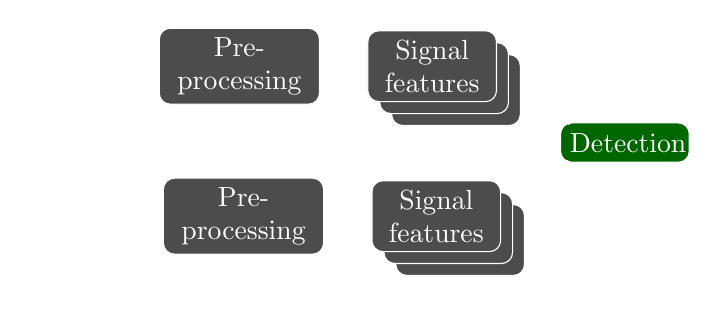
\begin{tikzpicture}[typetag/.style={rectangle, draw, rounded corners,fill=black!70, fill opacity=1, text opacity=1,text width=1.4cm, align=center,minimum width=1cm, minimum height=0.5cm},
    cascaded/.style={double copy shadow={shadow xshift=1ex,shadow yshift=-1ex}},color=white]
        % Nodes
        \node (input1) {$\hat{z}^n_1(t)$};
        \node [right=of input1,typetag,xshift=-0.4cm,text width=1.8cm] (preproc1) {Pre-processing};
        \node [right=of preproc1,typetag,cascaded,xshift=-0.4cm] (signal1) {Signal features};
        
        
        \node (input2)[below=of input1,yshift=-0.3cm] {$\hat{z}^n_M(t)$};
        \node [right=of input2,typetag,xshift=-0.4cm,text width=1.8cm] (preproc2) {Pre-processing};
        \node [right=of preproc2,typetag,cascaded,xshift=-0.4cm] (signal2) {Signal features};
        
        \node [right=of signal1,typetag,yshift=-0.97cm,xshift=-0.2cm,fill=green!40!black] (detection) {Detection};
        \node [below=of signal2,yshift=0.8cm] (dummy) {};
        
        % Arrows
        \draw[->] (input1) -- (preproc1);
        \draw[->] (preproc1) -- (signal1);
        \draw[->] (signal1) -- (detection);
        \draw[->] (input2) -- (preproc2);
        \draw[->] (preproc2) -- (signal2);
        \draw[->] (signal2) -- (detection);
        \path (input1) -- node[auto=false]{\vdots} (input2);
        
        \node [right=of preproc1,typetag,cascaded,xshift=-0.4cm] (signal1) {Signal features};
        
        \end{tikzpicture}
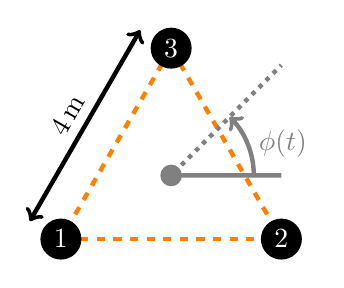
\begin{tikzpicture}[thick, scale=0.7]
    \node at (2,0) (LowerRight) {};
    \node at (-2,0) (LowerLeft) {};
    \node at (0,3.464) (Top) {};
    \node at (0,1.1547) (Center) {};
    \draw[orange, dashed,ultra thick] (LowerRight) -- (LowerLeft);
    \draw[orange, dashed,ultra thick] (LowerRight) -- (Top);
    \draw[orange, dashed,ultra  thick] (LowerLeft) -- (Top);
    \filldraw[black] (LowerLeft) circle (10pt) {};
    \node[white] at (LowerLeft) {$1$};
    \filldraw[black] (LowerRight) circle (10pt)  {};
    \node[white] at (LowerRight) {$2$};
    \filldraw[black] (Top) circle (10pt)  {};
    \node[white] at (Top) {$3$};

    \draw[black,ultra thick, <->,yshift=0.65*0.5cm,,xshift=-0.65*0.866cm] (-2,0) -- (0,3.464) node[midway,above,black,rotate=60] {$4$\,m};

    \filldraw[gray] (Center) circle (5pt) {};
    \draw[gray,ultra thick] (Center) -- (2,1.1547);
    \draw[gray,dotted,ultra thick] (Center) -- (2,1.1547+2);
    \draw[->, gray,ultra thick] (1.5,1.1547) arc
        [
            start angle=0,
            end angle= 45,
            x radius= 1.5cm,
            y radius =1.5cm
        ] node[midway,right,gray] {$\phi(t)$};
\end{tikzpicture}

\end{document}